\documentclass[10pt]{beamer}
\usetheme[
%%% options passed to the outer theme
%    hidetitle,           % hide the (short) title in the sidebar
%    hideauthor,          % hide the (short) author in the sidebar
%    hideinstitute,       % hide the (short) institute in the bottom of the sidebar
%    shownavsym,          % show the navigation symbols
%    width=2cm,           % width of the sidebar (default is 2 cm)
%    hideothersubsections,% hide all subsections but the subsections in the current section
%    hideallsubsections,  % hide all subsections
    left               % right of left position of sidebar (default is right)
%%% options passed to the color theme
%    lightheaderbg,       % use a light header background
  ]{AAUsidebar}

% If you want to change the colors of the various elements in the theme, edit and uncomment the following lines
% Change the bar and sidebar colors:
%\setbeamercolor{AAUsidebar}{fg=red!20,bg=red}
%\setbeamercolor{sidebar}{bg=red!20}
% Change the color of the structural elements:
%\setbeamercolor{structure}{fg=red}
% Change the frame title text color:
%\setbeamercolor{frametitle}{fg=blue}
% Change the normal text color background:
%\setbeamercolor{normal text}{bg=gray!10}
% ... and you can of course change a lot more - see the beamer user manual.


\usepackage[utf8]{inputenc}
\usepackage[english]{babel}
\usepackage[T1]{fontenc}
% Or whatever. Note that the encoding and the font should match. If T1
% does not look nice, try deleting the line with the fontenc.
\usepackage{helvet}

% colored hyperlinks
\newcommand{\chref}[2]{%
  \href{#1}{{\usebeamercolor[bg]{AAUsidebar}#2}}%
}

%custom setup
\graphicspath{{graphics/}}

\title[Cryptographic Protocol Verifier]% optional, use only with long paper titles
{An Efficient Cryptographic Protocol Verifier\\ Based on Prolog Rules}

\subtitle{Bruno Blanchet, 2001}  % could also be a conference name

\date{\today}

\author[Mikael Elkiær Christensen] % optional, use only with lots of authors
{
  Mikael Elkiær Christensen\\
  \href{mailto:michri11@student.aau.dk}{{\tt michri11@student.aau.dk}}
}
% - Give the names in the same order as they appear in the paper.
% - Use the \inst{?} command only if the authors have different
%   affiliation. See the beamer manual for an example

\institute[
%  {\includegraphics[scale=0.2]{aau_segl}}\\ %insert a company, department or university logo
  Dept.\ of Computer Science\\
  Aalborg University\\
  Denmark
] % optional - is placed in the bottom of the sidebar on every slide
{% is placed on the title page
  Department of Computer Science\\
  Aalborg University\\
  Denmark

  %there must be an empty line above this line - otherwise some unwanted space is added between the university and the country (I do not know why;( )
}


% specify a logo on the titlepage (you can specify additional logos an include them in
% institute command below
\pgfdeclareimage[height=1.5cm]{titlepagelogo}{AAUgraphics/aau_logo_new} % placed on the title page
%\pgfdeclareimage[height=1.5cm]{titlepagelogo2}{graphics/aau_logo_new} % placed on the title page
\titlegraphic{% is placed on the bottom of the title page
  \pgfuseimage{titlepagelogo}
%  \hspace{1cm}\pgfuseimage{titlepagelogo2}
}


\begin{document}
% the titlepage
{\aauwavesbg%
\begin{frame}[plain,noframenumbering] % the plain option removes the sidebar and header from the title page
  \titlepage
\end{frame}}

%%%%%%%%%%%%%%%%%%%%%%
\section{Introduction}

\begin{frame}
  \frametitle{The Problem}
    The Needham-Schroeder Public Key Protocol (1978):
    \begin{enumerate}
      \item $A \rightarrow S : A,B$
      \item $S \rightarrow A : \{K_b, B\}_{K_s^{-1}}$
      \item $A \rightarrow B : \{N_a, A\}_{K_b}$
      \item $B \rightarrow S : B,A$
      \item $S \rightarrow B : \{K_a, A\}_{K_s^{-1}}$
      \item $B \rightarrow A : \{N_a, N_b\textcolor{red}{, B}\}_{K_a}$
      \item $A \rightarrow B : \{N_b\}_{K_b}$
    \end{enumerate}
    \vfill
    Man-in-the-middle attack presented by Gabin Lowe (1995).
\end{frame}

\begin{frame}
  \frametitle{Not The Problem}
  \centering
  
\includegraphics[width=.5\textwidth]{heartbleed}\\
  (CVE-2014-0160)
\end{frame}

%%%%%%%%%%%%%%%%%%
\section{Overview}

\begin{frame}
  \frametitle{Overview}
  \begin{itemize}
    \item Previously: Applied $\pi$ Calculus, Multiset Rewriting, Model checking
    \begin{itemize}
      \item Limiting runs, inefficient, non-automatic, restrictions
    \end{itemize}
    \item Now: Prolog (First-order logic)
    \begin{itemize}
      \item FOL: Generally, \textbf{sound}, but not \textbf{complete}
      \item Uses custom resolution and unification
      \item Makes approximations
      \item Proves secrecy
    \end{itemize}
  \end{itemize}
\end{frame}

%%%%%%%%%%%%%%%%%%%%%%%%%%%%%%%%%
\section{Protocol representation}

\newcommand{\mytab}{\hspace{0.05\textwidth}}

\begin{frame}
  \frametitle{Syntax}
  \centering

  {\setlength{\tabcolsep}{20pt}
    \begin{tabular}{ll}
      $M, N ::=$ & terms \\
      \mytab$x$ & \mytab variable \\
      \mytab$a[M_1, \dots, M_n]$ & \mytab name \\
      \mytab$f(M_1, \dots, M_n)$ & \mytab function application \\\\

      $F ::=$ & fact \\
      \mytab$p(M_1, \dots, M_n)$ & \mytab predicate application \\\\

      $R ::=$ & rule \\
      \mytab$F_1 \land \dots \land F_n \rightarrow F$ & \mytab implication
    \end{tabular}
  }
\end{frame}

\newcommand{\fun}[1]{\textbf{#1}}

\begin{frame}
  \frametitle{Primitives}

  \begin{tabular}{lll}
    \multicolumn{2}{l}{$sk_A[]$, $sk_B[]$} \\
    \multicolumn{2}{l}{$k[x_1, \dots, x_n]$} \\[0.5em] \hline
    \textcolor{blue}{constructor} & \textcolor{blue}{destructor} \\
    $pk_A = \fun{pk}(sk_A[])$ & \\
    $\fun{pencrypt}(m, pk(sk))$ & $\fun{decrypt}(\fun{encrypt}(m, pk(sk)), sk) = m$ \\
    $\fun{sencrypt}(m, k)$ & $\fun{sdecrypt}(\fun{sencrypt}(m, k), k) = m$ \\
    $\fun{sign}(m, sk)$ & $\fun{getmess}(\fun{sign}(m, sk))$ \\
    $(\_, \dots, \_)$ & $\fun{\textit{i}th}((x_1, \dots, x_n)) = x_i | i \in \{1, \dots, n\}$ \\
    $h$ &
  \end{tabular}
\end{frame}

\begin{frame}
  \frametitle{Abilities of the attacker}

  Assumed the protocol is executed in the presence of an attacker that can:
  \begin{itemize}
    \item intercept all messages,
    \item compute new messages from the messages it has received, and
    \item send any message it can build.
  \end{itemize}
\end{frame}

\newcommand{\myvspace}{\\[0.5em]}

\begin{frame}
  \frametitle{Protocol}

  A protocol can be represented by three sets of rules:
  \begin{enumerate}
    \item Rules representing the computation abilities of the attacker \myvspace
      $attacker(x_1) \land ... \land attacker(x_n) \rightarrow attacker(f(x_1, \dots, x_n))$, \myvspace
      $attacker(M_1) \land \dots \land attacker(M_n) \rightarrow attacker(M)$ \myvspace
    \item Facts corresponding to initial knowledge of the attacker \myvspace
      $attacker(A[])$, $attacker(pk(sk_A[]))$ \myvspace
    \item Rules representing the protocol itself \myvspace
      $attacker(M_{j_1}) \land \dots \land attacker(M_{j_n}) \rightarrow attacker(M_i)$.
  \end{enumerate}
\end{frame}

\begin{frame}
  \frametitle{Approximations}

  \begin{itemize}
    \item New names are functions of messages previously received, unless altered.
    \item The same step of a protocol can be completed several times, yielding the same result, provided that the previous steps have been completed.\\[3em]
    \item Correctness still holds -- intuitively, more attacker options and safe, still safe with less options.
    \item However, can lead to false attacks.
  \end{itemize}
\end{frame}

\begin{frame}
  \frametitle{Multisets}

  \begin{itemize}
    \item A hypotheses $F_1, \dots, F_n$ of a rule are considered a multiset.
    \item A multiset of facts S is a function $S(F)$ yielding the number of repetitions of $F$ in $S$.
    \item Giving a point-wise order on functions: $S \subseteq S' \Leftrightarrow \forall F, S(F) \leq S'(F)$.
  \end{itemize}
\end{frame}

\begin{frame}
  \frametitle{Definition 1 (Rule Implication)}
  \centering

  $(H_1 \rightarrow C_1) \Rightarrow (H_2 \rightarrow C_2)$\\
  if and only if\\
  $\exists \sigma, \sigma C_1 = C_2, \sigma H_1 \subseteq H_2$
\end{frame}

\begin{frame}
  \frametitle{Definition 2 (Derivability)}

  \begin{columns}
    \begin{column}{.6\textwidth}
      Let $F$ be a closed fact.
      Let $B$ be a set of rules.
      $F$ is derivable from $B$ if and only if there exists a finite tree defined as follows:
      \begin{enumerate}
        \item Its nodes (except the root) are labelled by rules $R \in B$;
        \item Its edges are labelled by closed facts;
        \item If the tree contains a node labelled by $R$ with one incoming edge labelled by $F_0$ and $n$ outgoing edges labelled by $F_1, \dots, F_n$, then $R \Rightarrow \{F_1, \dots, F_n\} \rightarrow F_0$.
        \item The root has one outgoing edge, labelled by $F$.
      \end{enumerate}
    \end{column}
    \begin{column}{.4\textwidth}
      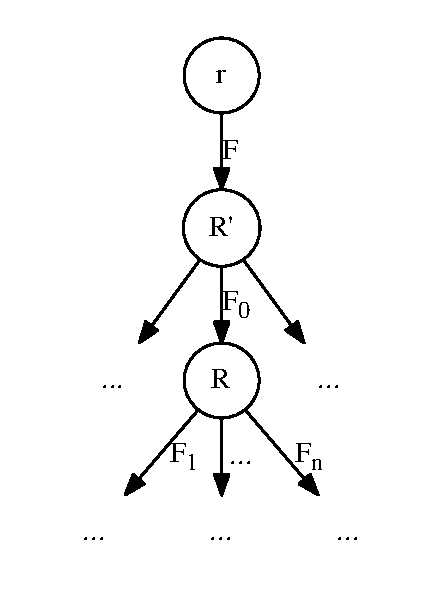
\includegraphics[width=\textwidth]{derivation_tree}
    \end{column}
  \end{columns}
\end{frame}

%%%%%%%%%%%%%%%%%%%%%%%%%%%
\section{Solving Algorithm}

\begin{frame}
  \frametitle{Prolog}
  \centering

  \begin{tabular}{l}
    $attacker(\fun{pencrypt}(m, \fun{pk}(sk))) \land attacker(sk)$ \\\mytab
    $\rightarrow attacker(m)$
  \end{tabular}
\end{frame}

\begin{frame}
  \frametitle{First phase: completion of the rule base}

  \begin{enumerate}
    \item For each $R \in B_0, B \leftarrow \fun{add}(\fun{elimdup}(R)B)$.
    \item Let $R \in B, R = H \rightarrow C$ and $R' \in B, R' = H' \rightarrow C'$.
      Assume that there exists $F_0 \in H'$ such that:
      \begin{itemize}
        \item[a)] $R \circ_{F_0} R'$ is defined;
        \item[b)] $\forall F \in H, F \in_r S$;
        \item[c)] $F_0 \not\in_r S$.
      \end{itemize}
      In this case, we execute\\
      \begin{center}
        $B \leftarrow \fun{add}(\fun{elimdup}(R \circ_{F_0} R'), B)$.
      \end{center}
      This procedure is executed until a fixed point is reached.
    \item Let $B' = \{(H \rightarrow C) \in B \forall F \in H, F \in_r S\}$.
  \end{enumerate}
\end{frame}

\begin{frame}
  \frametitle{Lemma 1 (Correctness of Phase 1)}
  \centering

  \parbox{.7\textwidth}{
    Let $F$ be a closed fact.
    $F$ is derivable from rules in $B_0$ if and only if $F$ is derivable from the rules in $B'$.
  }
\end{frame}

\begin{frame}
  \frametitle{Second phase: backward depth-first search}

  We define $\fun{derivablerec}(R,B'')$ by
  \begin{enumerate}
    \item $\fun{derivablerec}(R,B'') = Ø if \exists R' \in B'', R' \Rightarrow R$;
    \item $\fun{derivablerec}(Ø \rightarrow C, B'') = \{C\}$ otherwise;
    \item $\fun{derivablerec}(R, B'') = \cup \{\fun{derivablerec}(\fun{elimdup}(R' \circ_{F_0} R), \{R\} \cup B'') R' \in B', F_0$ such that $R' \circ_{F_0} R$ is defined $\}$ otherwise.
  \end{enumerate}
  \vspace{1em}
  $\fun{derivable}(F) = \fun{derivablerec}(\{F\} \rightarrow F, Ø)$.
\end{frame}

%%%%%%%%%%%%%%%%%
\section{Conclusion}

\begin{frame}
  \frametitle{Experimental results}
  \centering

  {\footnotesize
  \begin{tabular}{|l|l|r|r|}
    \hline
    Protocol & Result & \# Rules & Time (ms) \\ \hline
    Needham-Schroeder public key & Attack & 14 & 70 \\
    Needham-Schroeder public key corrected & Secure & 14 & 60 \\
    Needham-Schroeder shared key & Attack & 47 & 760 \\
    Needham-Schroeder shared key corrected & Secure & 51 & 1190 \\
    \multicolumn{4}{|c|}{} \\
    \multicolumn{4}{|c|}{\dots} \\
    \multicolumn{4}{|c|}{} \\ \hline
  \end{tabular}}
\end{frame}

%%%%%%%%%%%%
{\aauwavesbg
\begin{frame}[plain,noframenumbering]
  \finalpage{Time for questions...}
\end{frame}}

\end{document}
